\hypertarget{a00355}{}\section{Linked parameter update sequences}
\label{a00355}\index{Linked parameter update sequences@{Linked parameter update sequences}}
Sequence diagrams for some common linked parameter update scenarios. 

\hypertarget{a00355_advancedTopics_linkedParameters_sequences_contents}{}\subsection{On this page}\label{a00355_advancedTopics_linkedParameters_sequences_contents}
\begin{DoxyItemize}
\item \hyperlink{a00355_linkedParameters_sequences_user_gui}{User-\/generated update} \item \hyperlink{a00355_linkedParameters_sequences_automation}{Update from automation playback}\end{DoxyItemize}
\begin{DoxyNote}{Note}
To enable logging for these events at run time set {\ttfamily D\+T\+F\+\_\+\+A\+U\+T\+O\+M\+A\+T\+I\+O\+N=file@D\+T\+P\+\_\+\+L\+O\+W} in the \hyperlink{a00364}{Digi\+Trace} configuration file.
\end{DoxyNote}
\hypertarget{a00355_advancedTopics_linkedParameters_sequences_notes}{}\subsubsection{Notes on threading for these sequences}\label{a00355_advancedTopics_linkedParameters_sequences_notes}

\begin{DoxyItemize}
\item Calls from the host into \hyperlink{a00099}{A\+A\+X\+\_\+\+I\+Effect\+Parameters} may occur on any thread. In general, the only synchronization that is guaranteed for data model calls in these diagrams is that the call will follow whatever event is indicated as its trigger.
\item Calls from the host into \hyperlink{a00098}{A\+A\+X\+\_\+\+I\+Effect\+G\+U\+I} will occur on the main application thread unless indicated otherwise in the \hyperlink{a00098}{A\+A\+X\+\_\+\+I\+Effect\+G\+U\+I} documentation.
\item Host-\/driven updates to the algorithm context are always synchronized with the real-\/time processing thread
\end{DoxyItemize}

\begin{DoxySeeAlso}{See also}
\hyperlink{a00353}{Basic parameter update sequences}
\end{DoxySeeAlso}
\hypertarget{a00355_linkedParameters_sequences_user_gui}{}\subsection{User-\/generated update}\label{a00355_linkedParameters_sequences_user_gui}
This is the sequence of calls for a parameter update triggered by the user. For this sequence, we assume that the edit was triggered by a G\+U\+I event. Updates from control surfaces are handled in exactly the same way, except that the parameter touch, set value, and release tokens are generated by the control surface.

In this example the updated parameter is reciprocally linked to one other parameter. These are the \char`\"{}linker\char`\"{} and \char`\"{}linked\char`\"{} parameters, respectively.

This procedure is very similar to the non-\/linked case described \hyperlink{a00353_parameterUpdates_sequences_user}{here}. In the diagrams below, red arcs and pink section headings are used to indicate events that are specific to the linked parameter case.

Notes\+:
\begin{DoxyEnumerate}
\item This sequence shows the linked parameter reciprocally issuing a touch on the linker parameter. The touch fails since the linker parameter is already touched at this time. If the roles were reversed (if an edit occurred on the linked parameter) then this touch would succeed.
\item The host flags all set value tokens that are triggered by a plug-\/in within the scope of \hyperlink{a00061_a685858711efb8634ce66c327f2865c71}{A\+A\+X\+\_\+\+I\+Effect\+Parameters\+::\+Update\+Parameter\+Normalized\+Value()} \char`\"{}\+Update\+Parameter\+Normalized\+Value()\char`\"{}. When those set value tokens are processed they result in additional calls to \hyperlink{a00061_a685858711efb8634ce66c327f2865c71}{A\+A\+X\+\_\+\+I\+Effect\+Parameters\+::\+Update\+Parameter\+Normalized\+Value()} \char`\"{}\+Update\+Parameter\+Normalized\+Value()\char`\"{}. The host sets {\ttfamily i\+Source} to \hyperlink{a00206_a30be0398faf20c6b121239eb9399f3f7a401db669e68d5255c1126f7bf183b7ca}{A\+A\+X\+\_\+e\+Update\+Source\+\_\+\+Parameter} for each of these subsequent calls to indicate that the update originated from within a parameter update event.
\item \hyperlink{a00018_ae105f2a8a00facc2a190ef3ea86c5328}{Is\+Parameter\+Link\+Ready()} returns {\ttfamily true} during the linker parameter update because the update source is unknown and the parameter is touched. Both conditions must be true in order for the linking logic to proceed with setting linked parameters\textquotesingle{} values.
\item \hyperlink{a00018_ae105f2a8a00facc2a190ef3ea86c5328}{Is\+Parameter\+Link\+Ready()} returns {\ttfamily false} during the linked parameter update because the source is \hyperlink{a00206_a30be0398faf20c6b121239eb9399f3f7a401db669e68d5255c1126f7bf183b7ca}{A\+A\+X\+\_\+e\+Update\+Source\+\_\+\+Parameter}. This prevents update cycles for reciprocally linked parameters, as demonstrated here.
\end{DoxyEnumerate}\hypertarget{a00355_linkedParameters_sequences_user_gui_highLevel}{}\subsubsection{High-\/level interface calls and events}\label{a00355_linkedParameters_sequences_user_gui_highLevel}

\begin{DoxyImage}
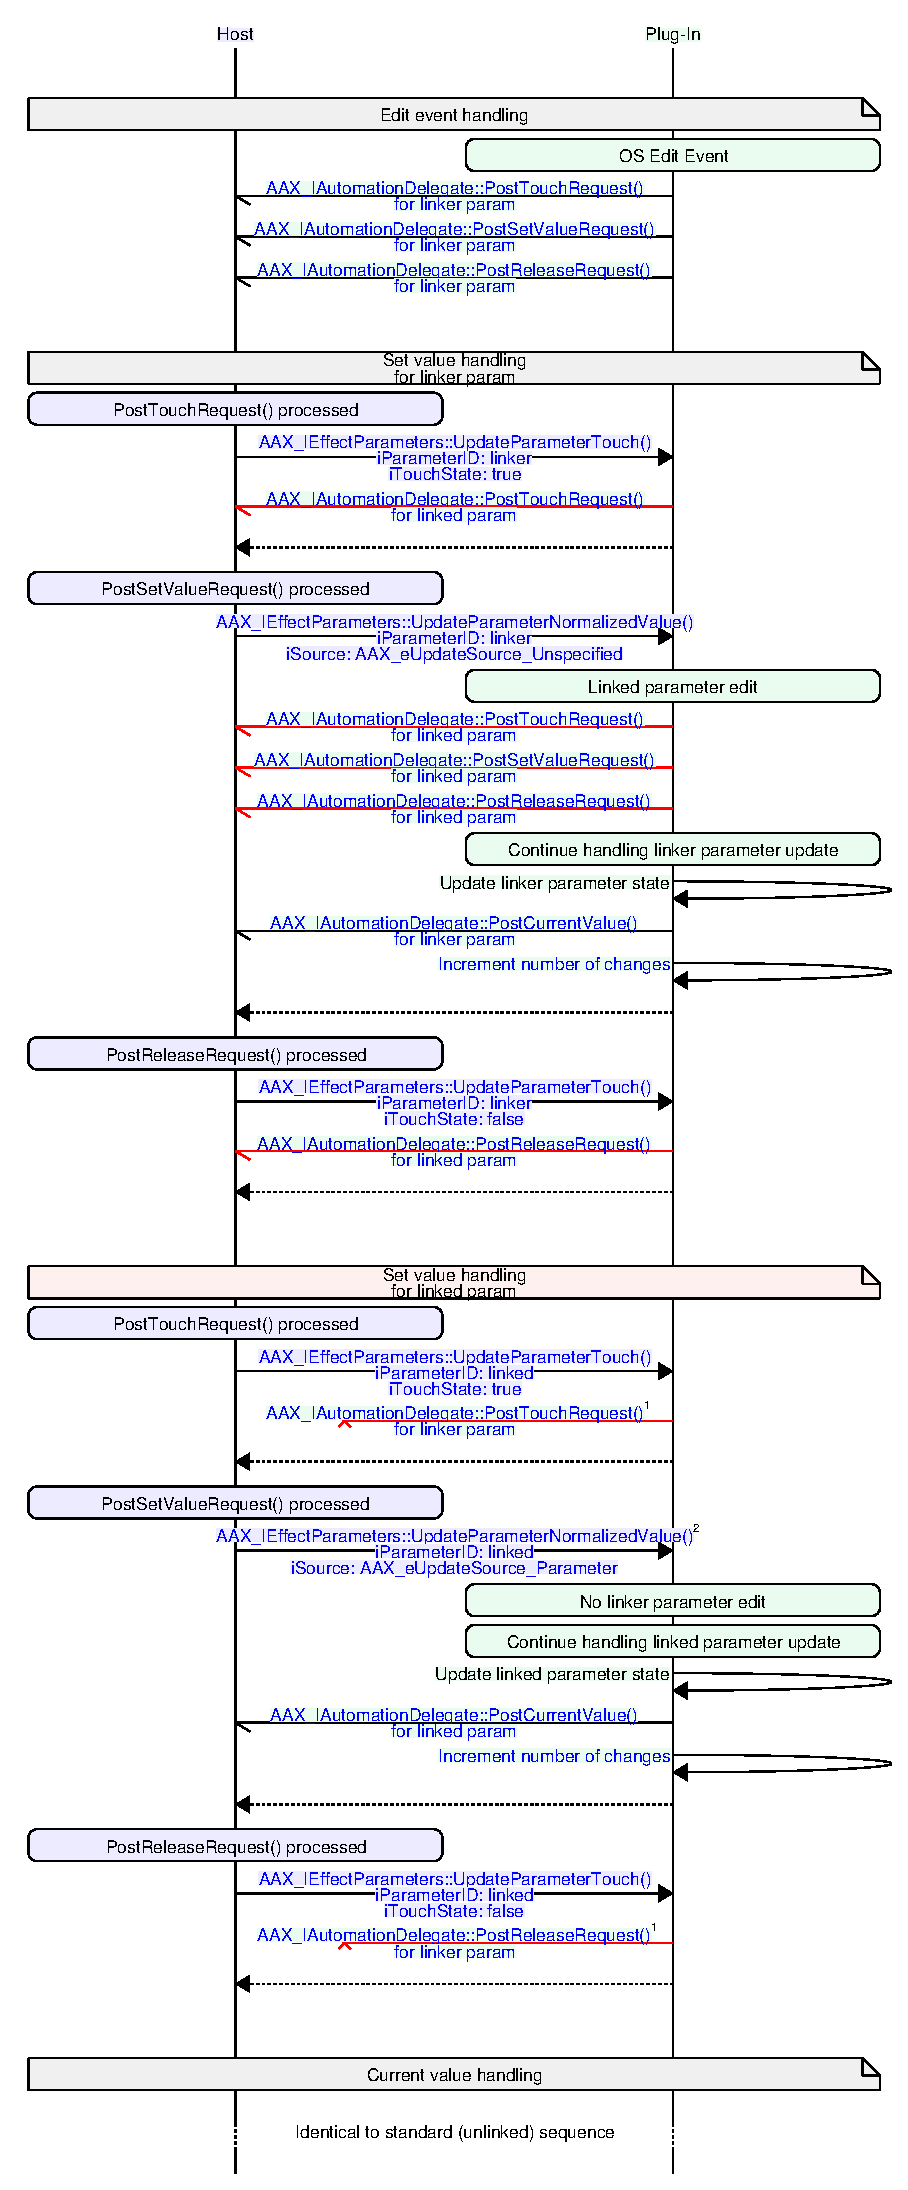
\includegraphics[width=\textwidth,height=\textheight/2,keepaspectratio=true]{msc_AAX_LinkedParameterUpdate_GUI_HighLevel}
\caption{High-\/level sequence of interface calls and events for a reciprocally linked parameter update following a user-\/generated edit}
\end{DoxyImage}
 \hypertarget{a00355_linkedParameters_sequences_user_gui_detail}{}\subsubsection{Detailed interface calls and events}\label{a00355_linkedParameters_sequences_user_gui_detail}
Note that this diagram assumes a G\+U\+I implementation that uses \hyperlink{a00061_a368b0f5a761d1eda4c41b420f153a077}{Set\+Parameter\+Normalized\+Value()}. The implementation could also use other parameter set methods, either in \hyperlink{a00099}{A\+A\+X\+\_\+\+I\+Effect\+Parameters} or directly on an \hyperlink{a00108}{A\+A\+X\+\_\+\+I\+Parameter}. The overall sequence would remain the same.


\begin{DoxyImage}
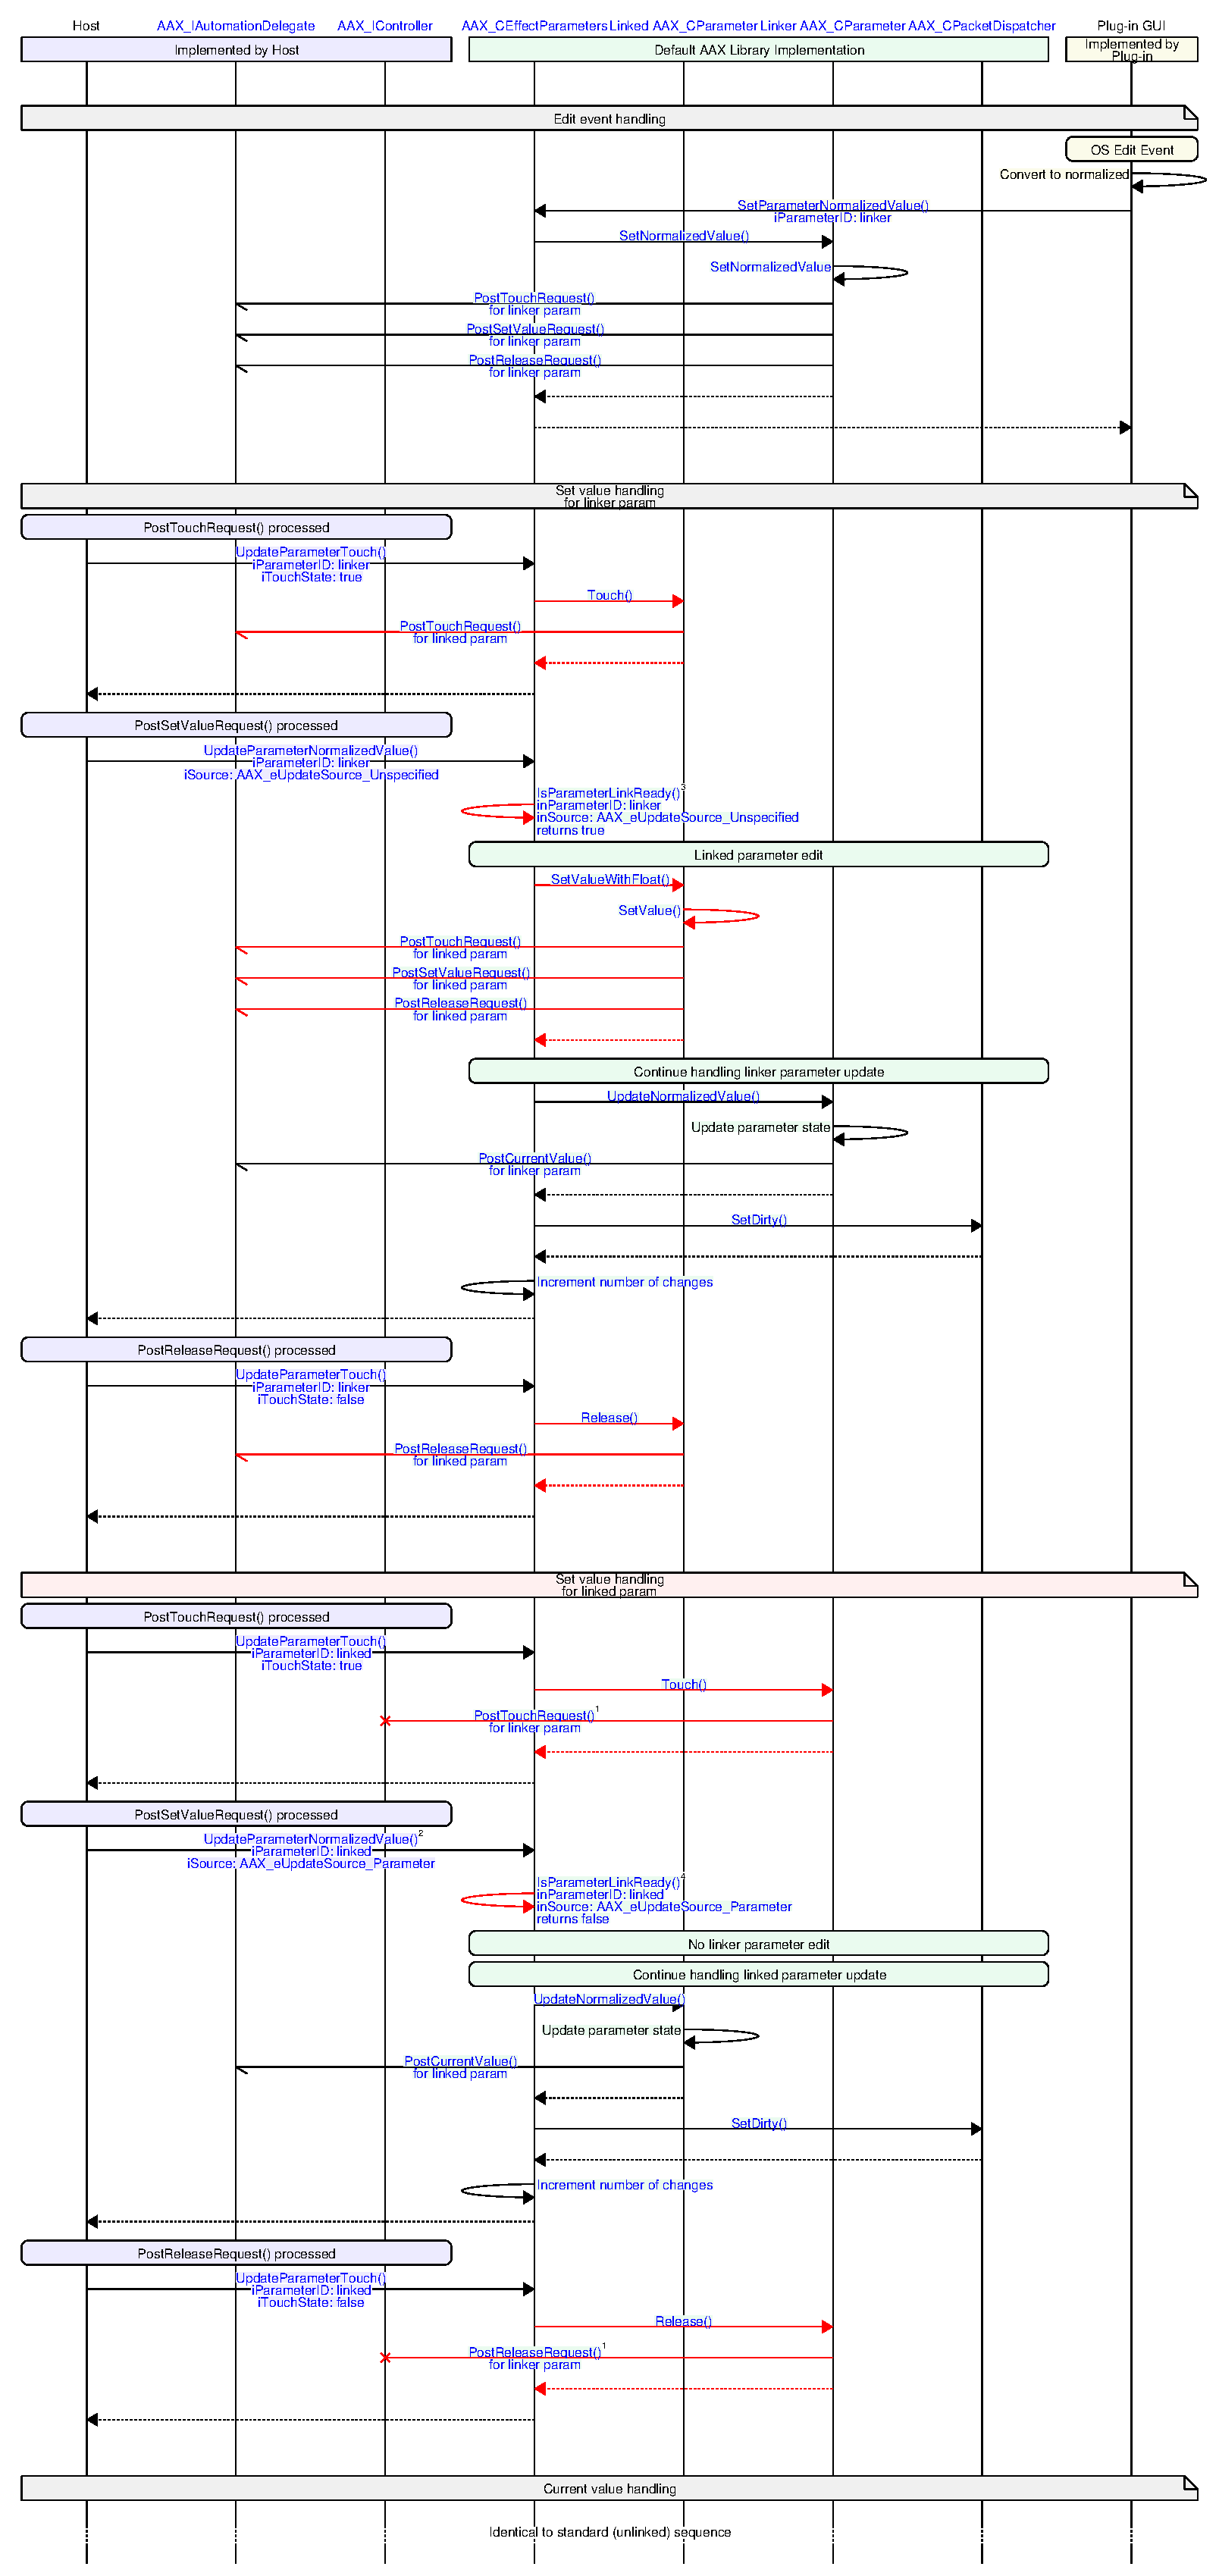
\includegraphics[width=\textwidth,height=\textheight/2,keepaspectratio=true]{msc_AAX_LinkedParameterUpdate_GUI}
\caption{Detailed sequence of method calls and events for a reciprocally linked parameter update following a user-\/generated edit on the plug-\/in G\+U\+I}
\end{DoxyImage}
 \hypertarget{a00355_linkedParameters_sequences_automation}{}\subsection{Update from automation playback}\label{a00355_linkedParameters_sequences_automation}
Since all parameter linking occurs while recording automation, automation playback is very simple. The automation lanes may contain any arbitrary values, so, in order to avoid fighting between incompatible values, the plug-\/in should respect all automation values during playback.

Notes\+:
\begin{DoxyEnumerate}
\item \hyperlink{a00018_ae105f2a8a00facc2a190ef3ea86c5328}{Is\+Parameter\+Link\+Ready()} returns {\ttfamily false} during automation playback because the updated parameter is not touched. This ensures that automation playback will proceed with the written values and also guarantees that the user will always be able to override the automation using a control surface encoder or G\+U\+I editor.
\end{DoxyEnumerate}


\begin{DoxyImage}
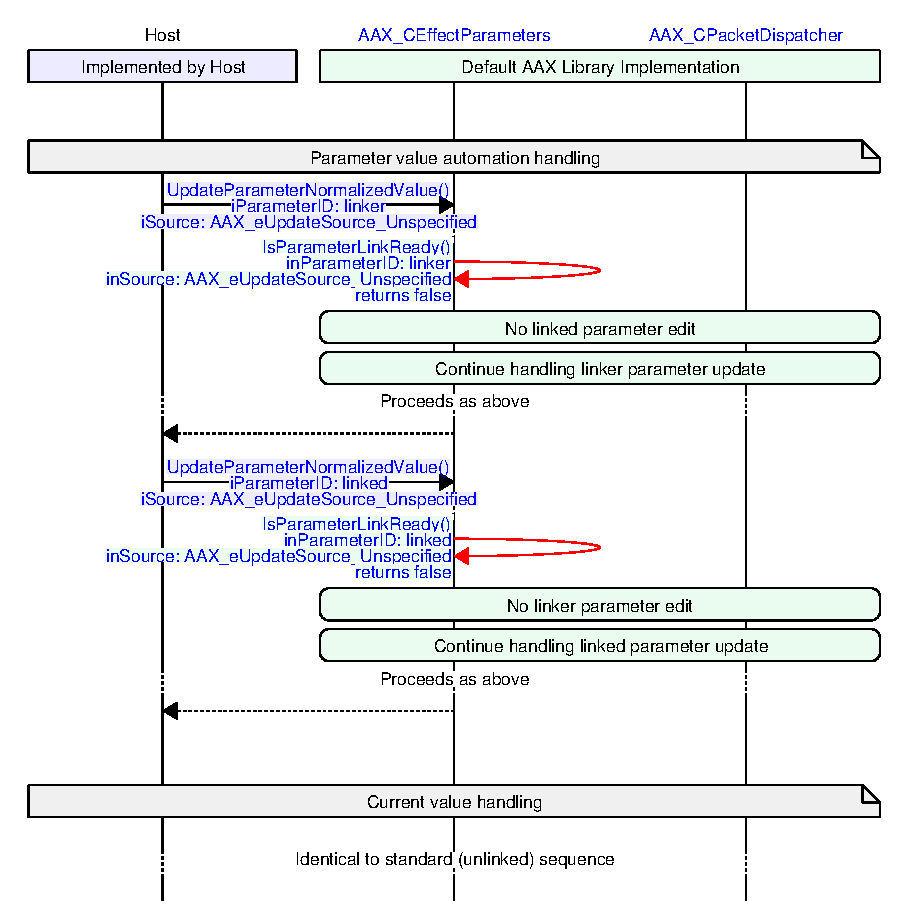
\includegraphics[width=\textwidth,height=\textheight/2,keepaspectratio=true]{msc_AAX_LinkedParameterUpdate_Automation}
\caption{Sequence of method calls and events during automation playback with linked parameters}
\end{DoxyImage}
Collaboration diagram for Linked parameter update sequences\+:
\nopagebreak
\begin{figure}[H]
\begin{center}
\leavevmode
\includegraphics[width=346pt]{a00355}
\end{center}
\end{figure}
